\subsection{Identifikation wesentlicher Energieeinsätze}

\subsubsection{Analyse und Unterscheidung von Energieeinsätzen}

Die DIN EN ISO 50001:2018-12 verpflichtet Organisationen im Rahmen der Planungsphase des PDCA-Zyklus zur Identifikation von wesentlichen Energieeinsätzen auf Grundlage 
der vorher durchgeführten Datenanalyse (\cite[S. 25]{DIN50001.2018}).
Die Norm definiert einen Energieeinsatz als Anwendung von Energie zum Beispiel für Energiedienstleistungen wie Lüftung oder Heizung, und bezeichnet den Begriff mitunter als 
Endnutzung von Energie (\cite[Kapitel 3.5.4]{DIN50001.2018}). 
Der Energieeinsatz ergibt sich aus dem Produkt des spezifischen Energieeinsatzes (Kehrwert der Energieeffizienz in Gleichung \eqref{EffizienzgleichungMiller}) 
und der Menge der Nachgefragten Energiedienstleistungen (\cite[S. 120]{Miller.2016}).
Mathematisch kann der Energieeinsatz mit den Gleichungen \eqref{EnergieeinsatzMiller} und \eqref{SepzifischerEnergieinsatzMiller} beschrieben werden.
\begin{equation}
    \text{Energieeinsatz} := \text{Spezifischer Energieeinsatz} \cdot \text{Menge Energiedienstleistung}
    \label{EnergieeinsatzMiller}
\end{equation}

\begin{equation}
    \text{Spezifischer Energieeinsatz} :=\frac{\text{Aufwand}}{\text{Erreichter Nutzen}}
    \label{SepzifischerEnergieinsatzMiller}
\end{equation}

Hat Beispielsweise eine Heizung in einem Büro mit 25 m² Grundfläche (Menge der Energiedienstleistung) einen Spezifischen Energieeinsatz von $100 \frac{\text{kWh}}{\text{m²}}$ pro Jahr 
bei definierter Sollinnentemperatur so beträgt der Jährliche Energieeinsatz der Heizung 2500 kWh.

Ein wesentlicher Energieeinsatz, auch SEU (en: significant energy use), wird von der Norm als Energieeinsatz der wesentlichen Anteil am Energieverbrauch 
hat und/oder erhebliches Potential für eine Verbesserung der energiebezogenen Leistung bietet definiert (\cite[Kapitel 3.5.6]{DIN50001.2018}). 
SEUs können Anlagen beziehungsweise Standorte, Systeme, Prozesse oder eine Einrichtungen sein (\cite[Kapitel 3.5.6]{DIN50001.2018}).
Zur Definition von Kriterien zur Identifikation von SEUs macht die Norm keine Angaben und verpflichtet die Organisation die die Norm anwendet zur Entscheidung was 
als wesentlicher Energieeinsatz anzusehen ist (\cite[S. 38]{DIN50001.2018}). 
Neben Energieerzeugungsanlagen und Umwandlungsanlagen gibt es Anlagenkategorien für Klimatisierungsanlagen, 
Lüftungsanlagen, Bleuchtungsanlagen sowie Informations- und Kommunikationstechnik (\cite[S. 14]{Hohnhold.2013}). 
Da sich die zuletzt genannten Anlagenkategorien mit den aus der DIN V 18599-1:2018-09 ermittelten Energiedienstleistungen für Organisationen des tertiären Wirtschaftssektors 
decken rückt die Analyse und Unterscheidung des Energieeinsatzes solcher Anlagen in den Fokus.
Die Disagggregation eines Bilanzraums nach Nutzengrößen wie sie in Abbildung \eqref{fig:Disagggregation_Bilanzraum_Nutzengrößen}  
dargestellt wird zeigt Potential auf durch die einzelne betrachtung der Zustandsgrößen eines Bilanzraums die Energieeinsätze der Energiedienstleistungen zu analysieren, 
unterscheiden und wesentliche Energieeinsätze unter den Energiedienstleistungen zu identifizieren. 

\begin{figure}[H]
    \centering
    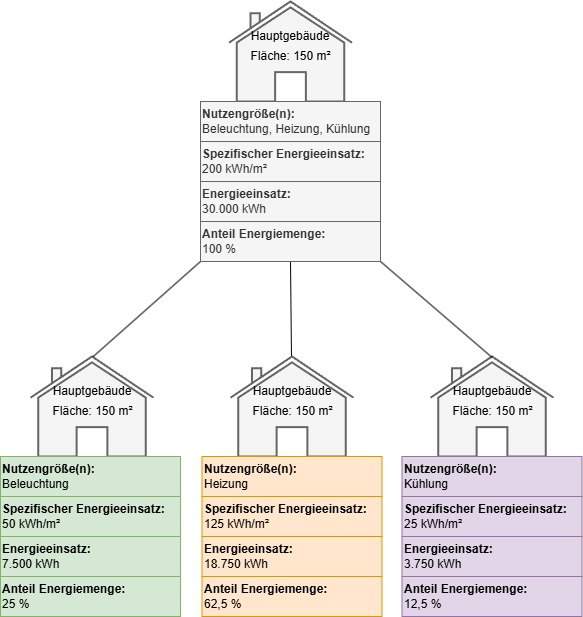
\includegraphics[width=1\textwidth]{../../Ressourcen/Abbildungen/Nutzengröße_Bewertungseinheit_Zerlegt_Beispiel.jpg}
    \caption{Beispiel: Disaggregation nach Nutzengrößen. (Eigene Darstellung)}
    \label{fig:Disagggregation_Bilanzraum_Nutzengrößen_Beispiel}
\end{figure}

Abbildung \eqref{fig:Disagggregation_Bilanzraum_Nutzengrößen_Beispiel} zeigt Beispielhaft wie das erarbeitete Konzept von Bilanzräumen zum erkennen von 
wesentlichen Energieeinsätzen beitragen kann. Wenn die aufwandsseitigen Ressourcen in einem festglegten Zeitintervall bekannt sind und die Nutzengröße durch eine 
Bewertungseinheit, wie in diesem Fall der Grundfläche in m², kann daraus mithilfe der Gleichung \eqref{SepzifischerEnergieinsatzMiller} der spezifische 
Energieeinsatz ermittelt werden. 
Unter Verwendung der Gleichung \eqref{EnergieeinsatzMiller} kann der Energieeinsatz im festglegten Zeitintervall berechnet werden und über den Anteil am 
gesamten Energieeinsatz von anderen Unterbilanzräumen unterschieden werden.
In diesem Beispiel macht die Heizungsanlage des Hauptgebäudes mit einem Energieeinsatz von 18.750 kWh 62,5 \% des Gesamtenergieverbrauchs aus und hat somit einen 
wesentlich Größeren Anteil am Gesamtenergieverbrauch als die Kühlungsanlage des Hauptgebäudes, welche mit einem Energieeinsatz von 3.750 kWh nur 12,5 \% des 
Gesamtenergieverbrauchs ausmacht.
Ob beim Energieeinsatz der Heizungsanlage ein erhebliches Potential für eine Verbesserung der energiebezogenen Leistung hat besteht hängt von den 
Anlagentechnischen Gegebenheiten der Heizung und den Gebäudetechnischen Gegebenheitung, wie Wärmedämmung ab.

Außerdem kann eine Analyse der Standorte beziehungsweise Gebäudezonen durch Disagggregation nach Untersuchungsgegenstand wie sie in 
\eqref{fig:Disagggregation_Bilanzraum_Untersuchungsgegenstand} visualisiert ist zur Identifikation wesentlicher Energieeinsätze durch die Analyse und Unterscheidung 
von Energieeinsätzen innerhalb von Gebäude(-zonen) beitragen.
\begin{figure}[H]
    \centering
    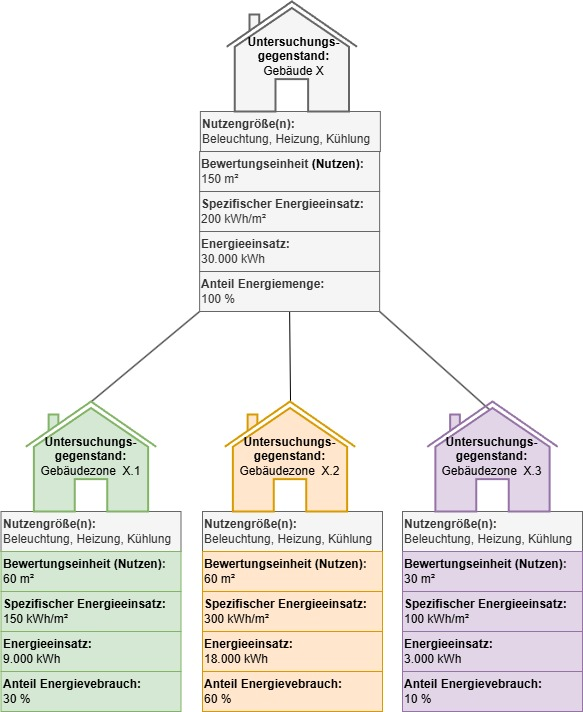
\includegraphics[width=1\textwidth]{../../Ressourcen/Abbildungen/Untersuchungsgegenstand_Zerlegt_Beispiel.jpg}
    \caption{Beispiel: Disaggregation nach Untersuchungsgegenstand. (Eigene Darstellung)}
    \label{fig:Disagggregation_Bilanzraum_Untersuchungsgegenstand_Beispiel}
\end{figure}
Abbildung \eqref{fig:Disagggregation_Bilanzraum_Untersuchungsgegenstand_Beispiel} visualisiert beispielhaft, wie eine Disagggregation des Untersuchungsgegenstands 
zur Analyse und Unterscheidung von Energieeinsätzen aus einer Perspektive des Standorts, also des Gebäudes und dessen Gebäudezonen, beitragen kann.
In diesem Beispiel macht die Etage 2 mit einem Energieeinsatz von 18.000 kWh 60\% des Gesamtenergieverbrauchs des Gebäudes aus während Etage 3 mit 
einem Energieeinsatz von 3.000 kWh nur 10\% des Gesamtenergieverbrauchs ausmacht.
Auch bei dieser Art der Disagggregation hängt das Potential für eine Verbesserung der energiebezogenen Leistung von den Gegebenheiten vor Ort ab.
Man sieht allerdings am Spezifischen Energieeinsatz, welcher die Größe der Grundfläche der Gebäudezonen mit einbezieht, dass in Etage 2 mit 300 kWh/m² 
im Verhältnis zu den anderen beiden Gebäudezonen ein hoher Spezifischer Energieeinsatz besteht. 
Das bedeutet dass Pro m² viel Energie verbraucht wird und kann ein Potential zur Verbesserung der energiebezogenen Leistung implizieren.

\subsubsection{Datengetriebene Ermittlung von Energieeinsätzen}
Um die Vorgaben der DIN EN ISO 50001:2018-12 zur ermittlung von Energieeinsätzen zu spezifizieren, betrachten wir die E DIN ISO 50006:2024-07,
welche sich mit der Messung der energiebezogenen Leistung im Rahmen der DIN EN ISO 50001:2018-12 befasst (\cite[S. 1]{DIN50006.2024}).
Organisationen sollen nach E DIN ISO 50006:2024-07 (Kapitel 5.1) Arten des Energieeinsatzes identifizieren und zum einen deren aktuellen, sowie früheren 
Energieverbrauch, zum anderen die aktuelle und frühere Energieeffizienz auf Basis von Messungen und anderen Daten bewerten. 
SEUs werden dann anhand der Analyse dieser Informationen, unter berücksichtigung von Faktoren die die energiebezogene Leistung beeinflussen, 
identifiziert (\cite[Kapitel 5.1]{DIN50006.2024}). 
Folglich ist eine Datengetriebene Analyse der Energieeinsätze notwendig, was Anforderungen an eine Messinfrastruktur in Organisationen impliziert.

\subsubsection{Energiefluss}
